\documentclass[hyperref={unicode}]{beamer}
\usepackage[utf8]{inputenc}
\usepackage[T1]{fontenc}
\usepackage[russian]{babel}
\usepackage{amsmath,mathrsfs,mathtext}
\usepackage{graphicx, epsfig}
\usepackage{multirow}
\DeclareGraphicsExtensions{.pdf,.png,.jpg}
\beamertemplatenavigationsymbolsempty % убрать снизу визуальный мусор
\usetheme{Warsaw}%{Warsaw}%{Singapore}%{Darmstadt}
\usecolortheme{default}%{sidebartab}%{beaver} %{wolverine}%{crane}%{sidebartab}
\definecolor{beamer@blendedblue}{RGB}{15,120,80}
%----------------------------------------------------------------------------------------------------------
\title[\hbox to 56mm{\hfill\insertframenumber\,/\,\inserttotalframenumber}]
{Применение активного обучения к графовым моделям на примере оценки рисков распространения эпидемии}
\author[А.\,Ю. Бишук]{\large \\Антон Юрьевич Бишук}
\institute{\large
Московский физико-технический институт}

\date{\footnotesize{Отчет по НИР/Группа 774, осень 2020\\\textbf{Научный руководитель:} Зухба Анастасия Викторовна}}
%----------------------------------------------------------------------------------------------------------
\begin{document}
%----------------------------------------------------------------------------------------------------------
\begin{frame}
%\thispagestyle{empty}
\titlepage
\end{frame}
%-----------------------------------------------------------------------------------------------------
\begin{frame}{Системы, описываемые графовыми моделями}

\begin{itemize}

\item Предполагается, что каждая вершина графа может находиться в конечном количестве состояний. 

\medskip

\item Состояние системы полностью определяется состоянием всех вершин.

\medskip


\item Текущее состояние известно только для части вершин. 


\medskip


\item Возможно запрашивать состояние отдельных вершин.

\medskip

\item Задача заключается в том, чтобы наиболее точно оценить состояние всей системы.

\medskip

\item Состояние системы меняется во времени в соответствии с определенными правилами.

% Здесь надо вслух сказать о эпидемиологических моделях на графах

\end{itemize}

 


\end{frame}
%----------------------------------------------------------------------------------------------------------
\begin{frame}{Цель исследования}

\medskip

\begin{block}{Цель работы}
Построить алгоритм, определяющий вершины, выяснение состояния которых позволят как можно точнее определить состояние всей системы с учетом изменения во времени.
% Важно, что с учетом изменения во времени. То есть не только кто кого уже заразил, но и кто кого заразит на следующем шаге
\end{block}

\begin{block}{Задачи}

\begin{itemize}
    \item Предложить возможные методы измерения количества информации о системе: в том числе примитивный (по количеству параметров) и энтропийный.
    \item Рассмотреть возможность использования предложенных методов для оценки полезности вершины с точки зрения информации о системе в целом.
    \item Изучить связь полученных методов с центральностями
    \item Выбрать подход к решению задачи
\end{itemize}
\end{block}

\end{frame}
%----------------------------------------------------------------------------------------------------------

\begin{frame}{Гипотезы}

Конкретизируем задачу: будем рассматривать графовые модели эпидемиологических процессов.

\bigskip

\begin{enumerate}
    \item Поиск нужных людей можно переформулировать в задачу поиска вершин с наибольшей центральность. Поэтому необходимо определить какие центральности можно для этого использовать.
    
    \medskip
    
    \item Поскольку мы имеем дело с не замкнутой системой, то наш алгоритм не должен быть детерминированным. Необходимо иногда делать случайные блуждания в графе.
    
\end{enumerate}
\end{frame}

%----------------------------------------------------------------------------------------------------------

\begin{frame}{Модель: обозначения}
\begin{enumerate}
    \item $i'$ -- статус $i$-го человека (0 -- здоров, 1 -- болен);
    \item $p_i$ -- вероятность того, что человек $i$ -- болен;
    \item $k_i$ -- число контактов $i$-го человека;
    \item $t_i^j$ -- время контакта $i$-го человека с $j$-ым.
    
    \vspace{1cm}
    Тогда во всей системе общее число параметров:
    
    $$n + 2\sum\limits_{i=1}^nk_i + 2\sum\limits_{i=1}^n[t_i]$$
\end{enumerate} 
\end{frame}
%**********************************************************************************
\begin{frame}{Модель: инициализация}
Инициализируем каждого пользователя вероятностью того, что он был на текущий момент зараженным.

Такой подход позволяет указывать заведомо больных и здоровых людей просто ставя вероятность болезни 1 и 0 соответственно.
\center{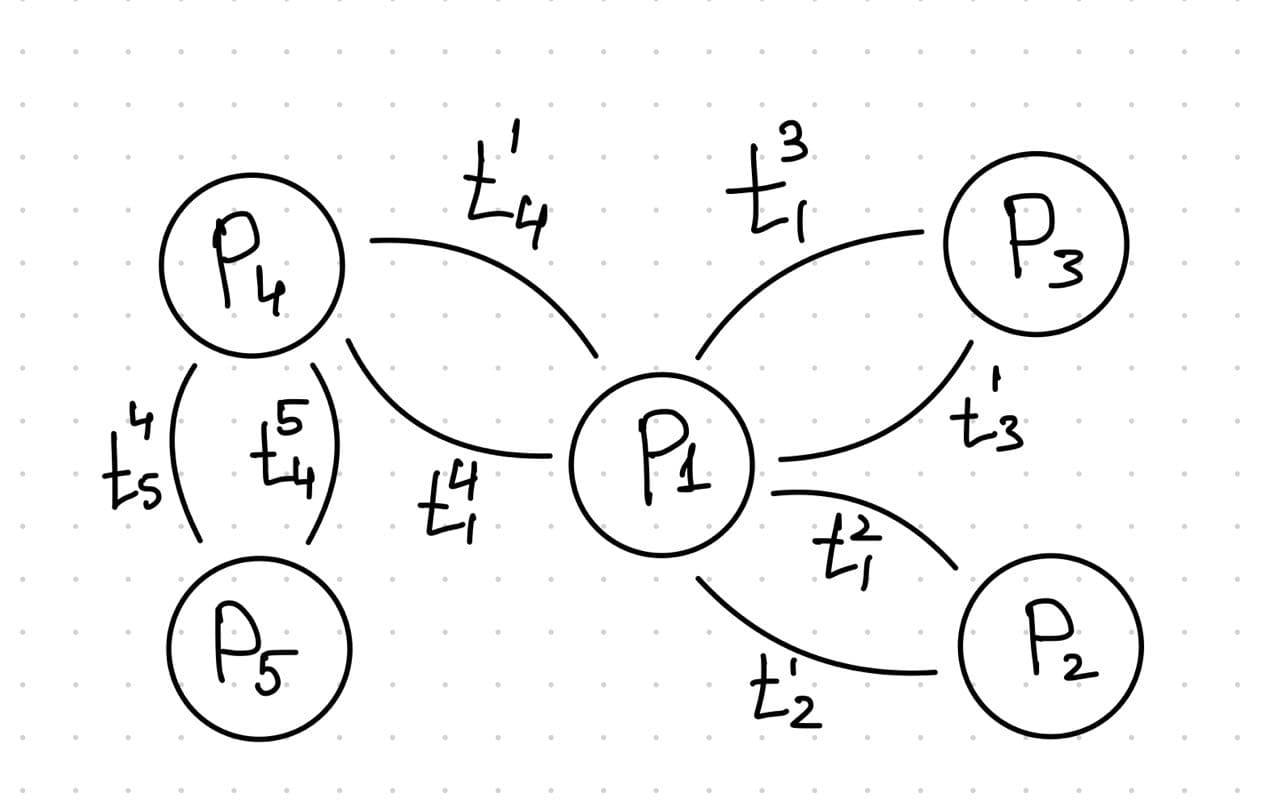
\includegraphics[width=0.5\linewidth]{1.jpg}\footnotesize \\}
\end{frame}
%*********************************************************************************
\begin{frame}{Модель: обновление параметров (1)}

$$f(t^2_1)=f(t^3_1)=f(t^4_1)=0$$

\center{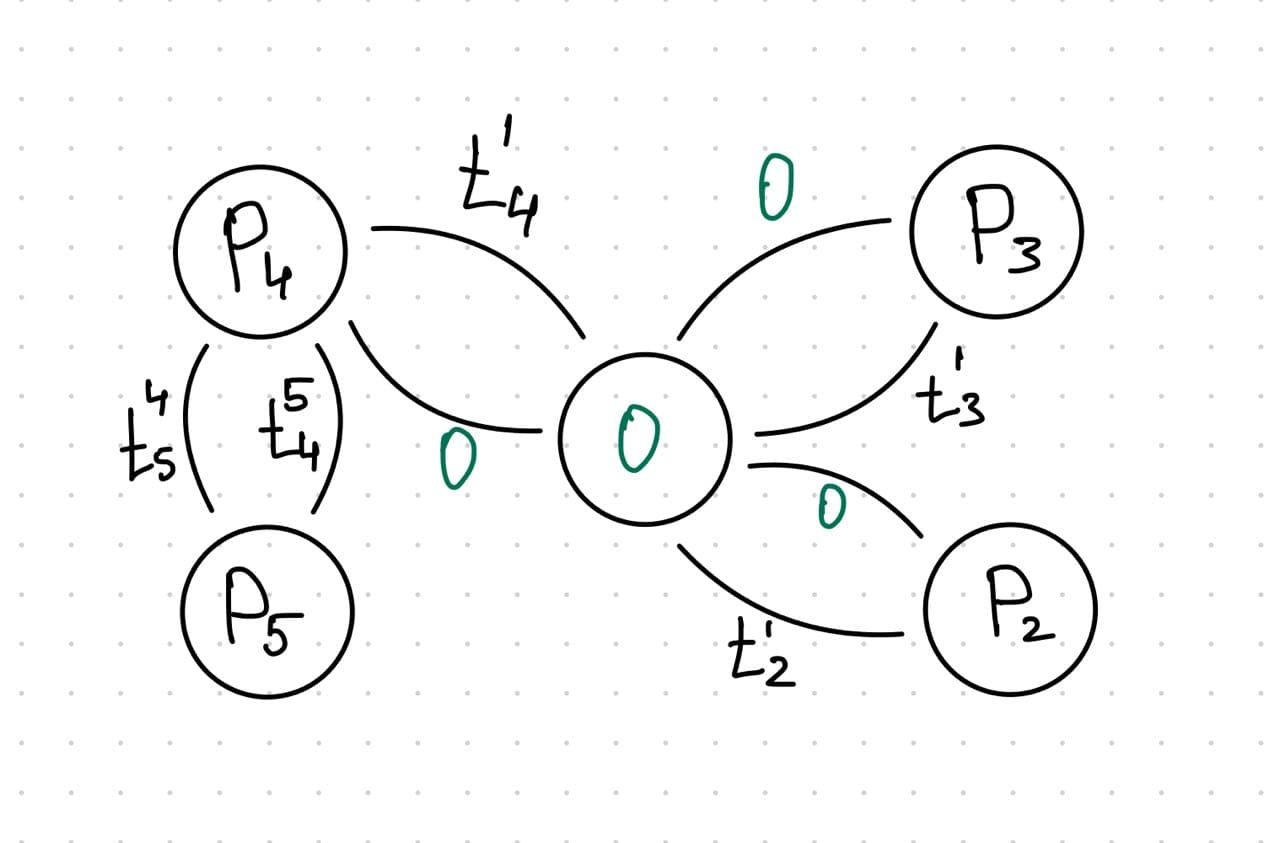
\includegraphics[width=0.5\linewidth]{2.jpg}\footnotesize \\ проверили человека и он оказался здоров, тогда граф на следующей итерации будет выглядеть следующим образом}

\end{frame}

\begin{frame}{Модель: обновление параметров (2)}

$$p_1' = 1 \text{ далее всегда}$$

На этого человека теперь так же не влияют другие.

\center{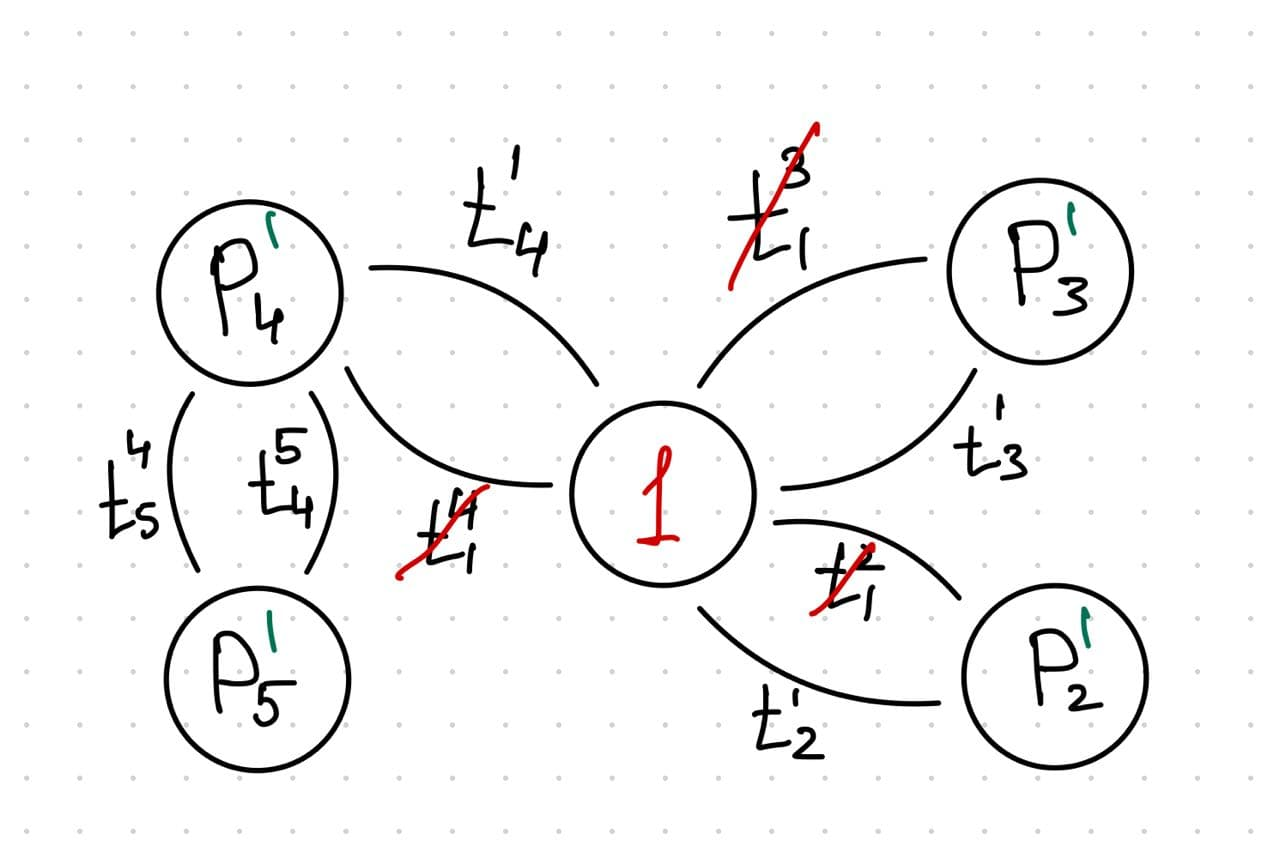
\includegraphics[width=0.5\linewidth]{4.jpg}\footnotesize \\ проверили человека и он оказался больным, тогда граф на следующей итерации будет выглядеть следующим образом}

\end{frame}

%*********************************************************************************
\begin{frame}{Вывод из модели}
\begin{enumerate}
    \item Если мы проверили $i$-го человека и он оказался здоров, то мы определили $k_i+[t_i]$ параметров системы;
    \item Если мы проверили $i$-го человека и он оказался болен, то мы определили $1 + 2k_i+[t_i]$ параметров системы;
\end{enumerate}

Тогда мы получаем, что:

\begin{equation*}
 \begin{cases}
   \text{с вероятностью }$p_i$ & \text{определим }$1+2k_i + [t_i]$ параметров \\
   \text{с вероятностью }$1-p_i$ & \text{определим }$k_i + [t_i]$ параметров
 \end{cases}
\end{equation*}

\end{frame}

%\begin{frame}{Выбор метрики}
%Задачу можно переформулировать на языке теории информации. Вся система имеет свою энтропию. При проверки пользователя мы уменьшаем её. При этом чем больше параметров мы своим выбором определяем, тем сильнее уменьшится энтропия всей системы.
%\end{frame}



%*********************************************************************************
\end{document} 